\documentclass{article}

\usepackage{amsfonts}
\usepackage{amsmath}
\usepackage{amssymb}
\usepackage{amsthm}
\usepackage{bookmark}
\usepackage{cancel}
\usepackage{extramarks}
\usepackage{fancyhdr}
\usepackage{floatrow}
\usepackage{forest}
\usepackage{graphicx}
\usepackage{hyperref}
\usepackage{listings}
\usepackage{mathrsfs}
\usepackage{proof}
\usepackage{pythonhighlight}
\usepackage[doublespacing]{setspace}
\usepackage{textcomp}
\usepackage{tikz}
\usepackage{wrapfig}
\usepackage{xparse}
\usepackage{xstring}
\usepackage{mathtools}
\usepackage{indentfirst}

\usepackage[backend=biber]{biblatex}
\addbibresource{APPMProject.bib}

\usetikzlibrary{automata,positioning}

%
% Basic Document Settings
%

\topmargin=-0.45in
\evensidemargin=0in
\oddsidemargin=0in
\textwidth=6.5in
\textheight=9.0in
\headsep=0.25in

\linespread{1.1}

\pagestyle{fancy}



\lhead{\textit{APPM 4350}}
\rhead{Final Project}
\lfoot{\lastxmark}
\cfoot{\thepage}

\renewcommand\headrulewidth{0.4pt}
\renewcommand\footrulewidth{0.4pt}

% \setlength\parindent{0pt}



 

%
% Title Page
%

\title{
	
}

\author{\hmwkAuthorName}
\date{}

%
% Various Helper Commands and Formatting Directives
%

\doublespacing

\allowdisplaybreaks

\title{Propagation of Voltage in a Neuron}
\author{Jamie George, Francesca Sica, Eric Wilkinson}
\date{December 7, 2020}

\begin{document}

\begin{titlepage} % Suppresses displaying the page number on the title page and the subsequent page counts as page 1
	\newcommand{\HRule}{\rule{\linewidth}{0.5mm}} % Defines a new command for horizontal lines, change thickness here
	
	\center % Centre everything on the page
	
	%------------------------------------------------
	%	Headings
	%------------------------------------------------
	
	\textsc{\LARGE University of Colorado Boulder}\\[1.5cm] % Main heading such as the name of your university/college
	
	\textsc{\Large APPM 4350}\\[0.5cm] % Major heading such as course name
	
	\textsc{\large Methods in Applied Mathematics: Fourier Series and Boundary Value Problems}\\[0.5cm] % Minor heading such as course title
	
	%------------------------------------------------
	%	Title
	%------------------------------------------------
	
	\HRule\\[0.4cm]
	
	{\huge\bfseries Propagation of Voltage in a Neuron}\\[0.4cm] % Title of your document
	
	\HRule\\[1.5cm]
	
	
	\begin{minipage}{0.4\textwidth}
		\begin{flushleft}
			\large
			\textit{Authors}\\
			\textsc{Jamie George}\\
			\textsc{Francesca Sica}\\
			\textsc{Eric Wilkinson}\\
		\end{flushleft}
	\end{minipage}
~
	
	\vfill\vfill\vfill 
	
	{\large December 7, 2020} 
	
	\vfill % Push the date up 1/4 of the remaining page
	
\end{titlepage}


\pagebreak

\begin{abstract}
In this project we analyze the propagation of voltage spikes in neurons using a partial differential equation known as the cable equation. We first consider the cable equation for a passive membrane, deriving Green's function and the voltage behaviour. Following this, we derive traveling wave solutions for the cable equation, determining the threshold and stability. Considering the equations we derived, we find that the cable equation is useful when modeling voltage spike propagation within a neuron.
\end{abstract}


\section{Introduction}
\subsection{Motivation}
In this project, we look at the propagation of voltage within a neuron. Voltage in neurons takes the form of action potentials, spikes in voltage which allow for communication between neurons. The propagation of voltage within a neuron can be described by a partial differential equation known as the cable equation. To find the cable equation, we use the idea that each part of an axonal membrane can be thought of as a component in an electrical circuit, as Hodgkin and Huxley showed in their Nobel Prize winning work.

\subsection{Model Derivation}
 To derive the cable equation we start with the current per unit length passing through the membrane, $J_{m}$, given in terms of voltage $v$
 \begin{gather*}
     J_{m}(x) = \frac{\partial}{\partial x} \left( \frac{1}{R(x)}\frac{\partial v}{\partial x} \right)
 \end{gather*}
 where $R(x) = R_{i}(x) + R_{e}(x)$. Using Ohm's law, V = IR, we define the internal and external currents on an infinitesimal segment of membrane $[x,x+dx]$. This results in the two equations
 \begin{gather*}
     v_{i}(x+dx) - v_{i}(x) = - I_{i}(x)R_{i}dx \textrm{ and } v_{e}(x+dx) - v_{e}(x) = - I_{e}(x)R_{e}dx
 \end{gather*}
 Dividing by $dx$ and then taking the limit $\lim_{dx\to0}$ gives the equations
 \begin{gather}  \label{eqns:Is}
     I_{i}(x) = -\frac{1}{R_{i}(x)}\frac{\partial v_{i}}{\partial x}\textrm{ and }I_{e}(x) = -\frac{1}{R_{e}(x)}\frac{\partial v_{e}}{\partial x}
 \end{gather}
 Using Kirchoff's Current Law, these two currents can be balanced with the current over the membrane, giving the equation
 \begin{gather*}
     I_{e}(x+dx) - I_{e}(x) = J_{m}(x)dx = I_{i}(x) - I_{i}(x+dx)
 \end{gather*}
 Again diving by $dx$ and taking the limit $\lim_{dx\to0}$ gives the equation:
 \begin{gather}  \label{eqns:Jm_in_I}
     J_{m}(x) = \frac{\partial I_{e}}{\partial x} = - \frac{\partial I_{i}}{\partial x}
 \end{gather}
 Now Eq. \ref{eqns:Is} are substituted into the equation for the total axial current, $I_{a} = I_{i} + I_{e}$. Using Ohm's law and the fact that $v = v_{i} - v_{e}$, we can rewrite the equation into
 \begin{gather*}
     I_{a} = I_{i} + I_{e} \Rightarrow \frac{R_{e}I_{a}}{R_{i} + R_{e}} = - \frac{1}{R_{i}}\frac{\partial v_{i}}{\partial x} + \left( \frac{1}{R_{i} + R_{e}} \right)\frac{\partial v}{\partial x}
 \end{gather*}
 Because $I_{a}$ is a constant, we can rearrange the terms and take $\frac{\partial}{\partial x}$ to get the equation
 \begin{gather*}
     \frac{\partial}{\partial x} \left[ \frac{1}{R_{i}(x)}\frac{\partial v_{i}}{\partial x} \right] = \frac{\partial}{\partial x} \left[ \left ( \frac{1}{R_{i}(x) + R_{e}(x)} \right) \frac{\partial v}{\partial x} \right] - I_{a} \frac{\partial}{\partial x} \left[ \frac{R_{e}(x)}{R_{i}(x) + R_{e}(x)} \right]
 \end{gather*}
 It is then assumed that the resistances are constant ($R_{e}(x) \equiv \bar{R_{e}}$ and $R_{i}(x) \equiv \bar{R_{i}}$). Applying Eq. \ref{eqns:Is} and \ref{eqns:Jm_in_I} gives the equation
 \begin{gather} \label{eqns:Jm_in_v}
     J_{m}(x) = \frac{\partial}{\partial x} \left( \frac{1}{R}\frac{\partial v}{\partial x} \right)
 \end{gather}
 
 Now considering the time variable as well, the current across the membrane per unit length $J_{m}(x,t)$ is given by the sum of the capacitive current, $J_{C}(x,t)$, the outward ionic current, $J_{ION}(v(x,t),t)$, and the inwardly applied current, $J_{A}(x,t)$. This gives the equation
 \begin{gather*}
     J_{m}(x,t) = J_{C}(x,t) + J_{ION}(v(x,t),t) - J_{A}(x,t)
 \end{gather*}
 Substituting in $J_{C}(x,t) = C\frac{\partial v}{\partial t}$ along with Eq. \ref{eqns:Jm_in_v} gives
 \begin{equation*}
     C\frac{\partial v(x,t)}{\partial t} = - J_{ION}(v(x,t),t) + \frac{1}{R}\frac{\partial^2 v(x,t)}{\partial x^2} + J_{A}(x,t)
 \end{equation*}
 A change of variables is then preformed to cancel $C$ and $R$ where $x \mapsto \frac{y}{\sqrt{R}}$ and $t \mapsto Cs$. The ionic currents are also assumed to be defined by function $f(v(y,s))$, a function of the rescaled voltage that accounts for multiple possible stable states. This gives the cable function
 \begin{gather*}
     \frac{\partial v(y,s)}{\partial s} = \frac{\partial^2v(y,s)}{\partial y^2}-f(v(y,s)) + J_{ext}(y,s)
 \end{gather*}
 This is then put back into the original variables for ease of use
 \begin{gather}  \label{eqns:cable}
    \frac{\partial v(x,t)}{\partial t} = \frac{\partial^2v(x,t)}{\partial x^2}-f(v(x,t)) + J_{ext}(x,t)
\end{gather}
 

\section{Passive Membrane}
We first consider the cable equation for a passive membrane. The current in a passive membrane flows according Ohm's law. That is, since $V_{ION} = I_{ION}R_{ION}$ we can write $I_{ION} = \frac{V_{ION}}{R_{ION}}$. Assuming Eq. \ref{eqns:cable} can be rescaled for unity, $f(v) = -v$. This means the cable equation may be simplified to the nonhomogeneous PDE
\begin{gather*}
    \frac{\partial v(x,t)}{\partial t} = \frac{\partial^2v(x,t)}{\partial x^2}-v(x,t) + J_{ext}(x,t)
\end{gather*}
We use this PDE to find stationary and generalized solutions to the passive membrane case by utilizing Fourier transforms and Green's function. For these solutions we consider an infinitely long cable because neural axons tend to be significantly longer than they are wide. 

\subsection{Stationary Solution}
We first find the stationary solutions that satisfy $V_t(x,t)=0$. Moreover, if we assume that $J_{ext}(x,t) \equiv 0$ we obtain the homogeneous ODE 
\begin{gather*}
    \frac{d^2V_0(x)}{d x^2} = V_0(x)
\end{gather*}
To solve for the stationary solutions, we let $V_0(x) = e^{rx}$, where $r$ is found to be $\pm1$, giving us the solution
\begin{gather*} 
V_0(x) = v_0e^{-x}+v_1e^{x}
\end{gather*}
The terms $v_0$ and $v_1$ are arbitrary constants. 

\subsection{Impulse Response}
For stationary input current localized at x = 0, we have $J_{ext}= \delta (x)$ and boundary conditions \\$lim_{x \Rightarrow \pm \infty}v(x,t) = 0$. In this case the stationary solutions are denoted as $V_F(x)$ and we obtain the nonhomogeneous ODE
\begin{gather*}
    \frac{d^2V_F(x)}{dx^2}-V_F(x)=-\delta(x)
\end{gather*}
Applying the Fourier transform to this ODE and solving for $\hat{V}_F(m)$ yields 
\begin{gather*}
    \hat V_F(m) = \frac{-1}{1+m^2}
\end{gather*}
The inverse Fourier transform \cite{fourierpairs} of $\hat{V}_F(m)$ yields
\begin{gather*} 
    V_F(x)=\frac{1}{2}e^{-|x|}
\end{gather*}

\subsection{Generalizing Solutions} 
For an arbitrary stationary input $J_{ext}(x)$ the  superposition principle for translated fundamental solutions is used to derive stationary solutions $V(x,t)=V_A(x)$. Green's function  approach to fundamental solutions \cite{greensfunc} is then used to find $V_A(x)$. To do this we define the linear operator $L_x=\frac{d^2}{dx^2}+1$. The linear operator $L_x$ takes the function $V_A(x)$ to $J_{ext}$. Green's function, $G(x-x_0)$, must then satisfy 
\begin{gather*}
    \frac{d^2G(x-x_0)}{dx^2}-G(x-x_0)=-\delta(x-x_0)
\end{gather*}
Thus the solution to Green's function is 
\begin{gather*}
    G(x-x_0)=\frac{1}{2}e^{-|x-x_0|}
\end{gather*}
Finally, we find the solution for arbitrary stationary input $J_{ext}(x)$ to be 
\begin{gather*}
    V_A(x)=\int\frac{1}{2}e^{-|x-x_0|}J_{ext}(x_0)dx_0
\end{gather*}

\subsection{Green's Function}
\subsubsection{Green's Function on the Infinite Cable}
The fundamental solution to the Cable equation for $\delta$-impulse at $t=0$ and $x=0$ is found by solving the PDE 
\begin{gather*}
    \frac{\partial v(x,t)}{\partial t}=\frac{\partial^2v(x,t)}{\partial x^2}-v(x,t)+\delta(t)\delta(x)
\end{gather*}
We use Fourier transform methods to find
\begin{gather*}
    v(x,t)=\frac{e^{\frac{(ix)^2}{4t}}}{2\pi e^t\sqrt{t}}\int_\infty^\infty e^{-u^2}du=\frac{e^{-(\frac{x^2}{4t}+t)}}{2\sqrt{\pi t}}=G_\infty(x,t)
\end{gather*}
This solution, denoted $G_{\infty}(x,t)$, is Green's function on the infinite cable.
\subsubsection{Voltage Behavior}
For fixed t we find

\begin{figure}[H]
\centering
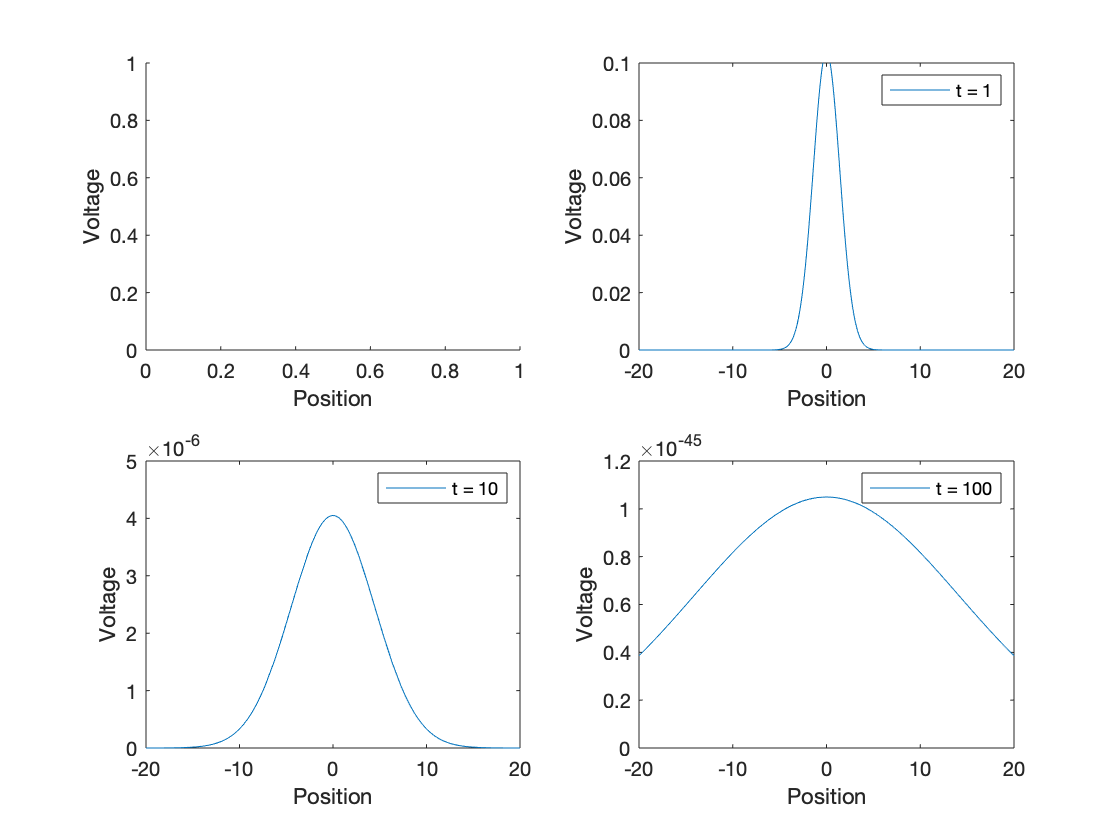
\includegraphics[width=0.75\textwidth]{fig1.png}
\caption{Voltage with Fixed t}
\label{fig:greens}
\end{figure}


We determine the voltage monotonicity by differentiating $G_{\infty}(x,t)$ with respect to t.  
At $x=0$ we find the voltage to be monotone decreasing for $t \in (0, \infty)$ as $\frac{d}{dt}G_{\infty}(0,t) \leq 0$ for all $t \in (0,\infty)$  
At $x=2$, the voltage is nonmonotonic because $\frac{d}{dt}G_{\infty}(0,t)$ takes both positive and negative values for $t \in (0, \infty)$.
Finally, we compute the total voltage for all x:
\begin{gather*} 
\overline{G}_\infty(t)=\int_{-\infty}^\infty G_\infty(x,t)dx=e^{-t}
\end{gather*}
Note that $\frac{d}{dt}e^{-t} \leq 0$ for all $t \in (0, \infty)$ so the total voltage is monotone decreasing for all t.

\subsection{Generalized Solutions}
Finally, we find the solution to the cable equation for any arbitrary spatiotemporal input $J_{ext}(x,t)$. Using the principle of superposition for translated functions, we find the solution to be 
\begin{gather*}
    V_A(x,t) = \int_{-\infty}^\infty\int_{-\infty}^\infty G_\infty (x-x_0,t-t_0)J_{ext}(x_0,t_0)dx_0dt_0
\end{gather*}
This is then solved for three different $J_{ext}(x,t)$ inputs; $1$, $sin(x)$, and $[\delta(x-1)\delta(x+1)]\delta(t)$. These solutions were then plotted against both $x$ and $t$ to understand the progression over time.

\begin{figure}[H]
\centering
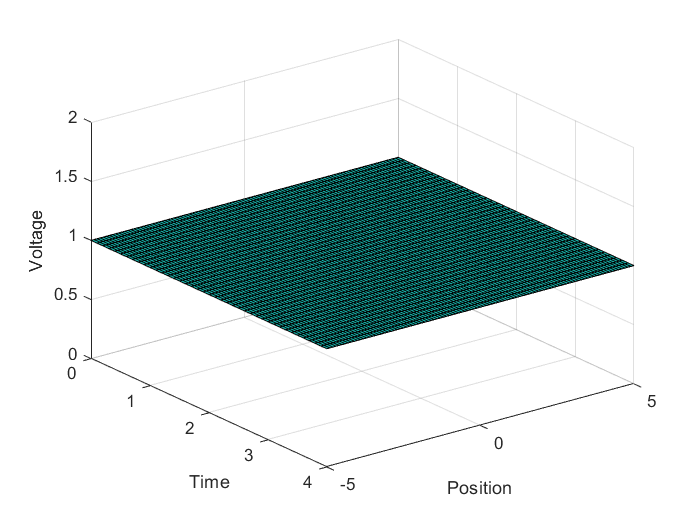
\includegraphics[width=0.75\textwidth]{fig4.png}
\caption{Voltage with respect to $x$ and $t$: $J_{ext}=1$}
\label{fig:gen_sol_1}
\end{figure}

\begin{figure}[H]
\centering
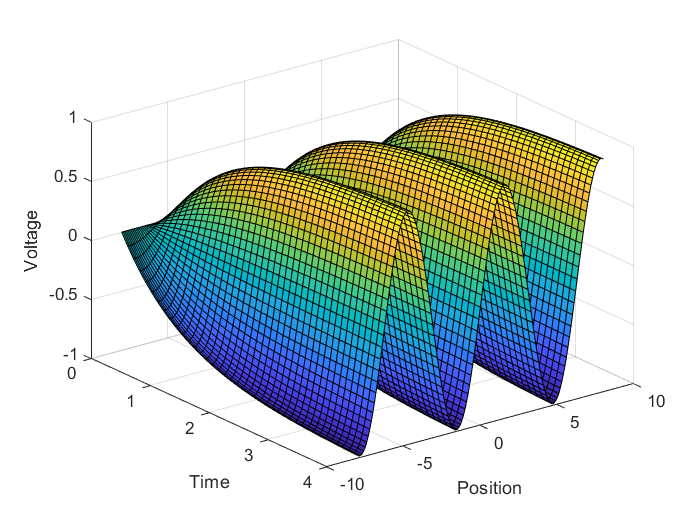
\includegraphics[width=0.75\textwidth]{fig5.png}
\caption{Voltage with respect to $x$ and $t$: $J_{ext}=sin(x)$}
\label{fig:gen_sol_sin}
\end{figure}

\begin{figure}[H]
\centering
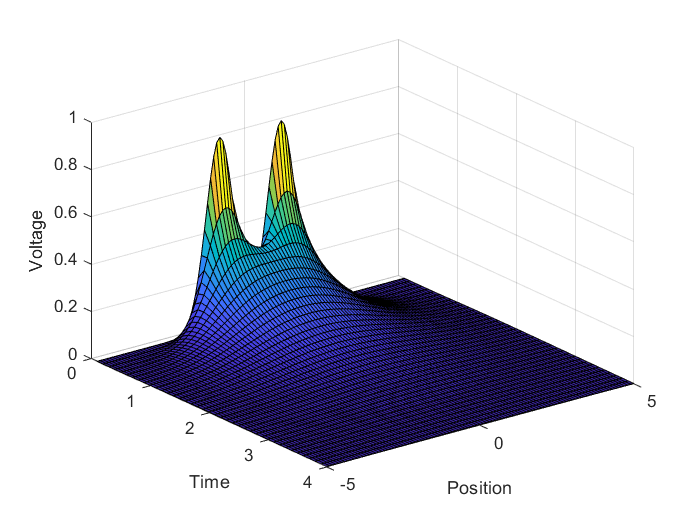
\includegraphics[width=0.75\textwidth]{fig3.png}
\caption{Voltage with respect to $x$ and $t$: $J_{ext}=[\delta(x-1)\delta(x+1)]\delta(t)$}
\label{fig:gen_sol_dirac}
\end{figure}

\section{Traveling Wave Solutions to the PDE}

Now we can look at modeling the "biological" neuron by incorporating active properties of a cell into the cable equation. To do so, we will assume a simple bistable membrane, with either $v = 1$ or $v = 0$. This is accomplished by choosing a form for $f(v(x,t))$ that allows the bistability. In this case, we used the given heavyside non-linearity
\begin{equation} \label{heavyside_eq}
    f(v)=-v+H(v-\theta)
\end{equation}

\subsection{Homogeneous Solutions} 
First we found the homogeneous solutions of Eq. \ref{heavyside_eq}, which are constant in space and time. We found that when $v>\theta$, $\bar{v}^+=1$ and when $v<\theta$, $\bar{v}^+=1$ $\bar{v}^-=0$. This means our two possible solutions are $v^+=1$ and $v^-=0$ where $v^-<\theta<v^+$.

\subsection{Change of Variables} 

Because the axon is modeled as infinitely long, physically possible solutions must then follow the boundary conditions
\begin{gather*}
\lim_{x \to\infty} \frac{\partial v(x,t)}{\partial x}=0
\textrm{ and }
\lim_{x \to-\infty} \frac{\partial v(x,t)}{\partial x}=0
\end{gather*}
We can use then use the boundary conditions and a change of variables to convert Eq. \ref{eqns:cable} to a second order ODE
\begin{gather*}
v(x,t)=V(\xi)
\textrm{ where }
\xi = x-ct\\
-cV'(\xi)=V''(\xi)+f(V(\xi))
\end{gather*}

\subsection{Traveling Front Solution} 

The second order ODE can be used to derive two ODEs
\begin{gather*} 
H(V(\xi)-\theta)=f(V(\xi)+V(\xi))=-cV'(\xi)-V''(\xi)+V(\xi)\\
V(\xi)>\theta \textrm{ when } \xi<0\\
V(\xi)<\theta \textrm{ when } \xi>0\\
-cV_+'(\xi)-V_+''(\xi)+V_+(\xi)=0, \xi \in (0,\infty)
    \begin{cases}
        \lim_{\xi \to\infty} V_+(\xi)=0\\
        \lim_{\xi \to\infty} V_+'(\xi)=0
    \end{cases}\\
-cV_-'(\xi)-V_-''(\xi)+V_-(\xi)=0, \xi \in (-\infty,0)
    \begin{cases}
        \lim_{\xi \to\infty} V_-(\xi)=1\\
        \lim_{\xi \to\infty} V_-'(\xi)=0
    \end{cases}
\end{gather*}

\subsection{Method of Undetermined Coefficients} 

The two ODEs are then solved using the method of undetermined coefficients to get the following equations
\begin{gather*} 
V_+(\xi)=Ae^{-\frac{1}{2}(\sqrt{c^2+4}+c)\xi}+Be^{\frac{1}{2}(\sqrt{c^2+4}-c)\xi}\\
V_-(\xi)=Ce^{-\frac{1}{2}(\sqrt{c^2+4}+c)\xi}+De^{\frac{1}{2}(\sqrt{c^2+4}-c)\xi}+1
\end{gather*}
Applying boundary conditions and solving for the constants results in the following solutions
\begin{gather*}
V_+(\xi)=(1-\frac{\sqrt{c^2+4}+c}{2\sqrt{c^2+4}})e^{-\frac{1}{2}(\sqrt{c^2+4}+c)\xi}\\
V_-(\xi)=-\frac{\sqrt{c^2+4}+c}{2\sqrt{c^2+4}}e^{\frac{1}{2}(\sqrt{c^2+4}-c)\xi}+1
\end{gather*}

\subsection{Threshold Condition} 
The speed, $c$, of the traveling front was found by applying the threshold condition $V(0)=\theta$.
\begin{gather*} 
c=\frac{1-2\theta}{\sqrt{\theta(1-\theta)}}
\end{gather*}
From this equation, we can see that $\theta$ is between zero and one. When $\theta$ is closer to zero, the neuron will be more active, and when $\theta$ is closer to one, the neuron is less active. 
\subsection{Traveling Front Solution Stability}
The traveling front solutions found should be asymptotically stable, meaning that if initial conditions start out near a traveling front solution they will converge to such a solution. We proved that these solutions are in fact asymptotically stable by using linear stability analysis. To begin, we added a perturbation to the traveling wave solution, derived an equation for its evolution, and checked if it decays in time. \\
First, we Taylor expand $f(V+\epsilon\psi)$ using the assumption that $\epsilon$ is small.
\begin{gather*} 
v(x,t)=V(\xi)+\epsilon\psi(\xi,t)\\
f(v)=-v+H(v-\theta)\\
f'(v)=-1+\delta(v-\theta)\\
f(v)\Big|_{\epsilon\psi=0}+(\epsilon\psi)f'(v)\Big|_{\epsilon\psi=0}=f(v_f)+\epsilon\psi f'(v_f)=-v_f+H(v_f-\theta)+\epsilon\psi(-1+\delta(v-\theta))
\end{gather*}
We then differentiate and use separation of variables to find the solutions below.
\begin{gather*}
\psi(\xi,t)=v'(\xi)\textrm{ when }\lambda=0\\
\psi(\xi,t)=e^{\lambda t}\overline{\psi}(\xi)\textrm{ when }\lambda<0\\
\textrm{No solution when }\lambda>0
\end{gather*}
Since the solutions decay in time, the solutions in the vicinity of the wave will tend to be attracted to it. This proves that the solutions are asymptotically stable. Additionally, there is no solutions when $\lambda>0$ because the $e$ term will blow up.

\section{Conclusions}
In this project we analyzed the cable equation to gain a deeper understanding of the propagation of voltage within a neuron. After providing background information and deriving the cable equation, we considered the equation for a passive membrane and derived solutions using Green's function. Following this, we examined neurons with bistable membranes and found traveling wave solutions for the cable equation. The findings made in this project showed us that partial differential equations and Fourier Series have a wide range of useful applications and are especially relevant to modeling neurons. In the future, we hope to learn how the mathematical modeling of a single neuron can be applied to networks or neurons.

\printbibliography[
heading=bibintoc,
title={References}
]

\newpage


\end{document}